Tous les angles sont orientés et confondus abusivement avec leur mesure principale.
\begin{enumerate}
	\item $\setgeo*{d}{1}$ et $\setgeo*{d}{2}$ sont deux demi-droites d'origine $F$ et telles que $\theta = \langle \setgeo*{d}{1} \,; \setgeo*{d}{2} \rangle \in \intervalO{0}{\dfrac{\pi}{2}}$ .

	\item $S$, le point de départ, est tel que $S \notin \setgeo*{d}{1} \cup \setgeo*{d}{2}$ et $\tau = \langle \setgeo*{d}{1} \,; [FS) \rangle \in \intervalO{0}{\theta}$ .
	
	\item Pour tout point $M$ du plan, nous noterons $H_M$ sont projeté orthogonal sur $\setgeo*{d}{2}$.
	
	\item Pour tout point $M$ qui est sur le trajet de la bille, mais pas sur $\setgeo*{d}{2}$, si $D_M$ est un point tel que $\vect{MD_M}$ indique la direction et le sens du trajet "sortant" de $M$, nous notons $\sigma_M = \langle \vect{MH_M} \,; \vect{MD_M} \rangle$.
\end{enumerate}


\medskip


\begin{center}
	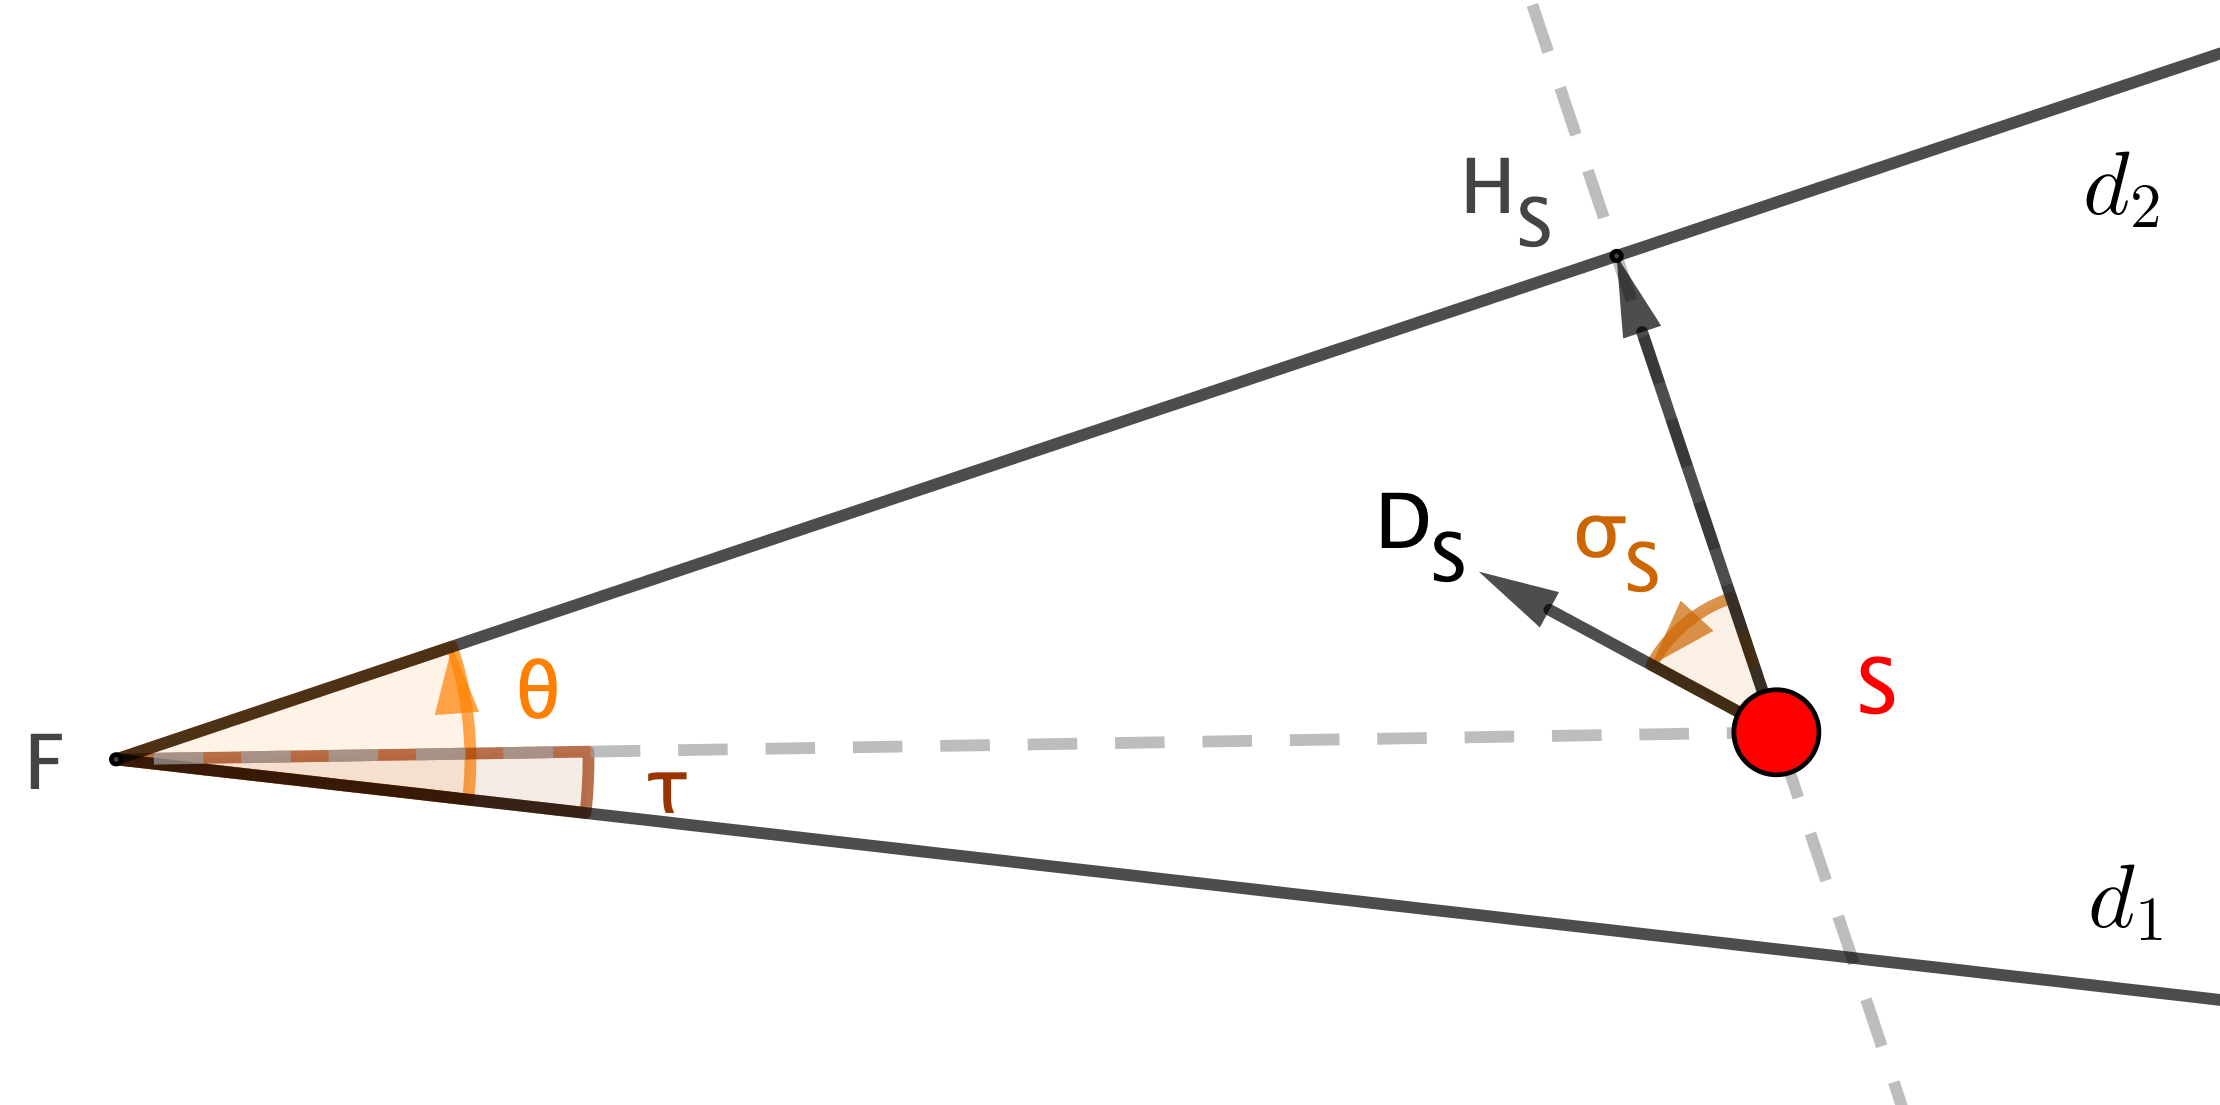
\includegraphics[width=12cm]{content/proof-notations.png}
	
	\itshape\small
	Notations pour la suite
\end{center}


